\section{系统业务需求}
当今社会,互联网蓬勃发展,我们正处于一个一切皆有可能的大变革时代,纸媒、微博、微信、APP正在随时随地地影响着人们的生活,舆情场也随之改变,社会化媒体尤其是微博成为舆情爆发的主要阵地,新媒体时代的舆情有以下特征:
广泛性:这是一个人人都有麦克风,人人都可以发言的时代。
碎片化:任何一个网民都有可能成为信息的生产者,舆论事件的报道者。舆论的发展呈网状扩散,加剧了信息的碎片性。
互动性:新媒体可以满足更多人的参与意识和表达愿望。
急速化:热点的传播速度很快,可以实现短时间内爆发式传播。
情绪化:新媒体时代网民有了自由发表意见的平台,但是难免鱼龙混杂,甚至存在偏激和非理性、群体盲从,情绪化现象严重。
泛娱乐化:泛娱乐化时代要时刻保持清醒的头脑,切勿让完全本能引导选择取向,警惕沦为娱乐的浅薄附庸。

新媒体舆情管理存在四大痛点:缺乏预警性、缺乏系统机制、严重的滞后性、缺乏影响力。
\begin{figure}[!htb]
	\centering
	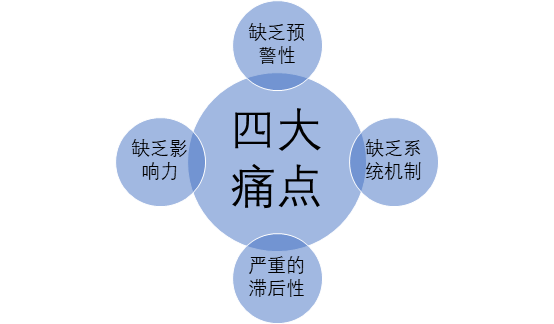
\includegraphics[scale=1]{image/b1.png}
	\caption{舆情管理的四大痛点}
\end{figure}
缺乏预警性:互联网已成为思想文化信息的集散地和社会舆论的放大器,做好新媒体公关舆情预警,根据舆情民意的趋势研判化解舆情危机是现阶段摆在舆情管理者面前的首要任务之一。
缺乏系统机制:新媒体环境下存在信息传递失真、传递不完全、解读失误等问题,降低了传播效能,不能取得预期的舆论引导效果。
严重的滞后性:新媒体具有全时、全域、全民、全速的传播特征。一旦有事件引发舆情危机,需要第一时间引起高度重视,做好严格统一的信息发布,并迅速表明态度,及时整改,尽可能与媒介做好深入沟通。
缺乏影响力:在新媒体时代,突发新闻事件一经发酵可能会迅速引起公众对企业或产品的质疑,如果不能在短期内有效解决舆情危机,就会使大众情绪进一步发酵。

大数据时代,对信息的加工是基础,对数据的解释是关键,对趋势的研判是目标,分众服务是方向。舆情研判强调大数据的关联性,发展和利用好数据资源是一场极大的舆情变革。因此,大数据与舆情监测与预警系统十分重要。目前国内经济社会转型发展环境压力加大,社会周期结构性突发舆情因素增多,加强大数据分析研判,获取情报,才能抓住机遇。
